\begin{enumerate}[label=\thechapter.\arabic*,ref=\thechapter.\theenumi]
\item Let $\{X_n\}_{n \geq 1}$ and Let $\{Y_n\}_{n \geq 1}$ be two sequences of random variables and $X$ and $Y$
be two random variables, all of them defined on the same probability space.
Which one of the following statements is true?
\begin{enumerate}[label=(\Alph*)]
\item If $\{X_n\}_{n \geq 1}$ converges in distribution to a real constant $c$, then $\{X_n\}_{n \geq 1}$
converges in probability to $c$.
\item If $\{X_n\}_{n \geq 1}$ converges in probability to $X$, then $\{X_n\}_{n \geq 1}$ converges in $3^{rd}$ mean
to $X$.
\item If $\{X_n\}_{n \geq 1}$ converges in distribution to $X$ and $\{Y_n\}_{n \geq 1}$ converges in
distribution to $Y$, then $\{X_n + Y_n\}_{n \geq 1}$ converges in distribution to $X+Y$.
\item If $\{E\brak{X_n}\}_{n \geq 1}$ converges to $E(X)$, then $\{X_n\}_{n \geq 1}$ converges in $1^{st}$ mean to $X$.
\end{enumerate}
\hfill (GATE ST 2023)
\iffalse
\let\negmedspace\undefined
\let\negthickspace\undefined
\documentclass[journal,12pt,twocolumn]{IEEEtran}
\usepackage{cite}
\usepackage{amsmath,amssymb,amsfonts,amsthm}
\usepackage{algorithmic}
\usepackage{graphicx}
\usepackage{textcomp}
\usepackage{xcolor}
\usepackage{txfonts}
\usepackage{listings}
\usepackage{enumitem}
\usepackage{mathtools}
\usepackage{gensymb}
\usepackage{comment}
\usepackage[breaklinks=true]{hyperref}
\usepackage{tkz-euclide} 
\usepackage{listings}
\usepackage{gvv}                                        
\def\inputGnumericTable{}                                 
\usepackage[latin1]{inputenc}                                
\usepackage{color}                                            
\usepackage{array}                                            
\usepackage{longtable}                                       
\usepackage{calc}                                             
\usepackage{multirow}                                         
\usepackage{hhline}                                           
\usepackage{ifthen}                                           
\usepackage{lscape}

\newtheorem{theorem}{Theorem}[section]
\newtheorem{problem}{Problem}
\newtheorem{proposition}{Proposition}[section]
\newtheorem{lemma}{Lemma}[section]
\newtheorem{corollary}[theorem]{Corollary}
\newtheorem{example}{Example}[section]
\newtheorem{definition}[problem]{Definition}
\newcommand{\BEQA}{\begin{eqnarray}}
\newcommand{\EEQA}{\end{eqnarray}}
\newcommand{\define}{\stackrel{\triangle}{=}}
\theoremstyle{remark}
\newtheorem{rem}{Remark}
\begin{document}

\bibliographystyle{IEEEtran}
\vspace{3cm}

\title{Probability Assignment}
\author{EE22BTECH11022-G.SAI HARSHITH$^{*}$% <-this % stops a space
}
\maketitle
\newpage
\bigskip
\renewcommand{\thefigure}{\theenumi}
\renewcommand{\thetable}{\theenumi}

Question: Let $\{X_n\}_{n \geq 1}$ and Let $\{Y_n\}_{n \geq 1}$ be two sequences of random variables and $X$ and $Y$
be two random variables, all of them defined on the same probability space.
Which one of the following statements is true?
\begin{enumerate}[label=(\Alph*)]
\item If $\{X_n\}_{n \geq 1}$ converges in distribution to a real constant $c$, then $\{X_n\}_{n \geq 1}$
converges in probability to $c$.
\item If $\{X_n\}_{n \geq 1}$ converges in probability to $X$, then $\{X_n\}_{n \geq 1}$ converges in $3^{rd}$ mean
to $X$.
\item If $\{X_n\}_{n \geq 1}$ converges in distribution to $X$ and $\{Y_n\}_{n \geq 1}$ converges in
distribution to $Y$, then $\{X_n + Y_n\}_{n \geq 1}$ converges in distribution to $X+Y$.
\item If $\{E\brak{X_n}\}_{n \geq 1}$ converges to $E(X)$, then $\{X_n\}_{n \geq 1}$ converges in $1^{st}$ mean to $X$.
\end{enumerate}
\fi
\solution 
\begin{enumerate}
\item $X_n$ converges in distribution to $X$, $X_n \xrightarrow{d} X$, then for all x,
\begin{align}
lim_{n \to \infty} F_{X_n}(x) &= F_X(x)
\end{align}
\item $X_n$ converges in probability to $X$, $X_n \xrightarrow{p} X$, then for all $\epsilon > 0$,
\begin{align}
lim_{n \to \infty} \pr{|X_n-X|>\epsilon}&=0
\label{eq:1}
\end{align}
\item $X_n$ converges in $p^{th}$ mean to $X$, then we have
\begin{align}
lim_{n \to \infty} E(|X_n-X|^p)&=0
\end{align}
\end{enumerate}
\begin{enumerate}[label=(\Alph*)]
\item For $\epsilon > 0$, $B$ be defined as
\begin{align}
B&=\{x: |x-c| \geq \epsilon\}
\end{align}
Now,
\begin{align}
\pr{|X_n-c| \geq \epsilon}&= \pr{X_n \in B}
\end{align}
Using Portmanteau Lemma, if $X_n \xrightarrow{d} c$, we have
\begin{align}
\limsup\limits_{n \to \infty}\pr{X_n \in B} & \leq \pr{c \in B}\\
& \leq \pr{|0-0|\geq \epsilon}\\
& \leq \pr{0\geq \epsilon}\\
& \leq 0\\
&=0\\
lim_{n \to \infty} \pr{|X_n-c|>\epsilon}&=0
\end{align}
From \eqref{eq:1}, $X_n \xrightarrow{p} c$. So, we have
\begin{align}
X_n \xrightarrow{d} c \implies X_n \xrightarrow{p} c
\end{align}
Option (A) is correct.
\item Statement (B) is may or may not correct.
Counter Example:
Consider distribution
\begin{table}[!ht]
	%%%%%%%%%%%%%%%%%%%%%%%%%%%%%%%%%%%%%%%%%%%%%%%%%%%%%%%%%%%%%%%%%%%%%%
%%                                                                  %%
%%  This is the header of a LaTeX2e file exported from Gnumeric.    %%
%%                                                                  %%
%%  This file can be compiled as it stands or included in another   %%
%%  LaTeX document. The table is based on the longtable package so  %%
%%  the longtable options (headers, footers...) can be set in the   %%
%%  preamble section below (see PRAMBLE).                           %%
%%                                                                  %%
%%  To include the file in another, the following two lines must be %%
%%  in the including file:                                          %%
%%        \def\inputGnumericTable{}                                 %%
%%  at the beginning of the file and:                               %%
%%        \input{name-of-this-file.tex}                             %%
%%  where the table is to be placed. Note also that the including   %%
%%  file must use the following packages for the table to be        %%
%%  rendered correctly:                                             %%
%%    \usepackage[latin1]{inputenc}                                 %%
%%    \usepackage{color}                                            %%
%%    \usepackage{array}                                            %%
%%    \usepackage{longtable}                                        %%
%%    \usepackage{calc}                                             %%
%%    \usepackage{multirow}                                         %%
%%    \usepackage{hhline}                                           %%
%%    \usepackage{ifthen}                                           %%
%%  optionally (for landscape tables embedded in another document): %%
%%    \usepackage{lscape}                                           %%
%%                                                                  %%
%%%%%%%%%%%%%%%%%%%%%%%%%%%%%%%%%%%%%%%%%%%%%%%%%%%%%%%%%%%%%%%%%%%%%%



%%  This section checks if we are begin input into another file or  %%
%%  the file will be compiled alone. First use a macro taken from   %%
%%  the TeXbook ex 7.7 (suggestion of Han-Wen Nienhuys).            %%
\def\ifundefined#1{\expandafter\ifx\csname#1\endcsname\relax}


%%  Check for the \def token for inputed files. If it is not        %%
%%  defined, the file will be processed as a standalone and the     %%
%%  preamble will be used.                                          %%
\ifundefined{inputGnumericTable}

%%  We must be able to close or not the document at the end.        %%
	\def\gnumericTableEnd{\end{document}}


%%%%%%%%%%%%%%%%%%%%%%%%%%%%%%%%%%%%%%%%%%%%%%%%%%%%%%%%%%%%%%%%%%%%%%
%%                                                                  %%
%%  This is the PREAMBLE. Change these values to get the right      %%
%%  paper size and other niceties.                                  %%
%%                                                                  %%
%%%%%%%%%%%%%%%%%%%%%%%%%%%%%%%%%%%%%%%%%%%%%%%%%%%%%%%%%%%%%%%%%%%%%%

	\documentclass[12pt%
			  ,landscape%
                    ]{report}
       \usepackage[latin1]{inputenc}
       \usepackage{fullpage}
       \usepackage{color}
       \usepackage{array}
       \usepackage{longtable}
       \usepackage{calc}
       \usepackage{multirow}
       \usepackage{hhline}
       \usepackage{ifthen}

	\begin{document}


%%  End of the preamble for the standalone. The next section is for %%
%%  documents which are included into other LaTeX2e files.          %%
\else

%%  We are not a stand alone document. For a regular table, we will %%
%%  have no preamble and only define the closing to mean nothing.   %%
    \def\gnumericTableEnd{}

%%  If we want landscape mode in an embedded document, comment out  %%
%%  the line above and uncomment the two below. The table will      %%
%%  begin on a new page and run in landscape mode.                  %%
%       \def\gnumericTableEnd{\end{landscape}}
%       \begin{landscape}


%%  End of the else clause for this file being \input.              %%
\fi

%%%%%%%%%%%%%%%%%%%%%%%%%%%%%%%%%%%%%%%%%%%%%%%%%%%%%%%%%%%%%%%%%%%%%%
%%                                                                  %%
%%  The rest is the gnumeric table, except for the closing          %%
%%  statement. Changes below will alter the table's appearance.     %%
%%                                                                  %%
%%%%%%%%%%%%%%%%%%%%%%%%%%%%%%%%%%%%%%%%%%%%%%%%%%%%%%%%%%%%%%%%%%%%%%

\providecommand{\gnumericmathit}[1]{#1} 
%%  Uncomment the next line if you would like your numbers to be in %%
%%  italics if they are italizised in the gnumeric table.           %%
%\renewcommand{\gnumericmathit}[1]{\mathit{#1}}
\providecommand{\gnumericPB}[1]%
{\let\gnumericTemp=\\#1\let\\=\gnumericTemp\hspace{0pt}}
 \ifundefined{gnumericTableWidthDefined}
        \newlength{\gnumericTableWidth}
        \newlength{\gnumericTableWidthComplete}
        \newlength{\gnumericMultiRowLength}
        \global\def\gnumericTableWidthDefined{}
 \fi
%% The following setting protects this code from babel shorthands.  %%
 \ifthenelse{\isundefined{\languageshorthands}}{}{\languageshorthands{english}}
%%  The default table format retains the relative column widths of  %%
%%  gnumeric. They can easily be changed to c, r or l. In that case %%
%%  you may want to comment out the next line and uncomment the one %%
%%  thereafter                                                      %%
\providecommand\gnumbox{\makebox[0pt]}
%%\providecommand\gnumbox[1][]{\makebox}

%% to adjust positions in multirow situations                       %%
\setlength{\bigstrutjot}{\jot}
\setlength{\extrarowheight}{\doublerulesep}

%%  The \setlongtables command keeps column widths the same across  %%
%%  pages. Simply comment out next line for varying column widths.  %%
\setlongtables

\setlength\gnumericTableWidth{%
	125pt+%
	125pt+%
	167pt+%
0pt}
\def\gumericNumCols{3}
\setlength\gnumericTableWidthComplete{\gnumericTableWidth+%
         \tabcolsep*\gumericNumCols*2+\arrayrulewidth*\gumericNumCols}
\ifthenelse{\lengthtest{\gnumericTableWidthComplete > \linewidth}}%
         {\def\gnumericScale{1*\ratio{\linewidth-%
                        \tabcolsep*\gumericNumCols*2-%
                        \arrayrulewidth*\gumericNumCols}%
{\gnumericTableWidth}}}%
{\def\gnumericScale{1}}

%%%%%%%%%%%%%%%%%%%%%%%%%%%%%%%%%%%%%%%%%%%%%%%%%%%%%%%%%%%%%%%%%%%%%%
%%                                                                  %%
%% The following are the widths of the various columns. We are      %%
%% defining them here because then they are easier to change.       %%
%% Depending on the cell formats we may use them more than once.    %%
%%                                                                  %%
%%%%%%%%%%%%%%%%%%%%%%%%%%%%%%%%%%%%%%%%%%%%%%%%%%%%%%%%%%%%%%%%%%%%%%

\ifthenelse{\isundefined{\gnumericColA}}{\newlength{\gnumericColA}}{}\settowidth{\gnumericColA}{\begin{tabular}{@{}p{125pt*\gnumericScale}@{}}x\end{tabular}}
\ifthenelse{\isundefined{\gnumericColB}}{\newlength{\gnumericColB}}{}\settowidth{\gnumericColB}{\begin{tabular}{@{}p{100pt*\gnumericScale}@{}}x\end{tabular}}
\ifthenelse{\isundefined{\gnumericColC}}{\newlength{\gnumericColC}}{}\settowidth{\gnumericColC}{\begin{tabular}{@{}p{200pt*\gnumericScale}@{}}x\end{tabular}}

\begin{tabular}[c]{%
	b{\gnumericColA}%
	b{\gnumericColB}%
	b{\gnumericColC}%
	}

%%%%%%%%%%%%%%%%%%%%%%%%%%%%%%%%%%%%%%%%%%%%%%%%%%%%%%%%%%%%%%%%%%%%%%
%%  The longtable options. (Caption, headers... see Goosens, p.124) %%
%	\caption{The Table Caption.}             \\	%
% \hline	% Across the top of the table.
%%  The rest of these options are table rows which are placed on    %%
%%  the first, last or every page. Use \multicolumn if you want.    %%

%%  Header for the first page.                                      %%
%	\multicolumn{3}{c}{The First Header} \\ \hline 
%	\multicolumn{1}{c}{colTag}	%Column 1
%	&\multicolumn{1}{c}{colTag}	%Column 2
%	&\multicolumn{1}{c}{colTag}	\\ \hline %Last column
%	\endfirsthead

%%  The running header definition.                                  %%
%	\hline
%	\multicolumn{3}{l}{\ldots\small\slshape continued} \\ \hline
%	\multicolumn{1}{c}{colTag}	%Column 1
%	&\multicolumn{1}{c}{colTag}	%Column 2
%	&\multicolumn{1}{c}{colTag}	\\ \hline %Last column
%	\endhead

%%  The running footer definition.                                  %%
%	\hline
%	\multicolumn{3}{r}{\small\slshape continued\ldots} \\
%	\endfoot

%%  The ending footer definition.                                   %%
%	\multicolumn{3}{c}{That's all folks} \\ \hline 
%	\endlastfoot
%%%%%%%%%%%%%%%%%%%%%%%%%%%%%%%%%%%%%%%%%%%%%%%%%%%%%%%%%%%%%%%%%%%%%%

\hhline{|-|-|-}
	 \multicolumn{1}{|p{\gnumericColA}|}%
	{\gnumericPB{\centering}\gnumbox{$X_n$}}
	&\multicolumn{1}{p{\gnumericColB}|}%
	{\gnumericPB{\centering}\gnumbox{0}}
	&\multicolumn{1}{p{\gnumericColC}|}%
	{\gnumericPB{\centering}\gnumbox{$n$}}
\\
\hhline{|---|}
	 \multicolumn{1}{|p{\gnumericColA}|}%
	{\gnumericPB{\centering}\gnumbox{$\pr{X_n}$}}
	&\multicolumn{1}{p{\gnumericColB}|}%
	{\gnumericPB{\centering}\gnumbox{$1-\frac{1}{n}$}}
	&\multicolumn{1}{p{\gnumericColC}|}%
	{\gnumericPB{\centering}\gnumbox{$\frac{1}{n}$}}
\\
\hhline{|-|-|-|}
\end{tabular}

\ifthenelse{\isundefined{\languageshorthands}}{}{\languageshorthands{\languagename}}
\gnumericTableEnd

\end{table}\\
For $\epsilon>0$, $X_n$ converges in probability to $X=0$
\begin{align}
lim_{n \to \infty} \pr{|X_n-X|>\epsilon}&=lim_{n \to \infty} \pr{X_n>\epsilon}
\end{align}
$X_n>\epsilon$vis subset of $X_n=n$ since every time $X_n$ equals n, it's also true that $X_n$ is greater than $\epsilon$. But there may be times when $X_n$ is greater than $\epsilon$ without $X_n$ being equal to n. So,
\begin{align}
\pr{X_n>\epsilon}&\leq \pr{X_n=n}\\
lim_{n \to \infty} \pr{|X_n-X|>\epsilon}&\leq lim_{n \to \infty} \pr{X_n=n}\\
&\leq lim_{n \to \infty} \frac{1}{n}\\
& \leq 0\\
&=0
\end{align} 
But $X_n$ does not converges in $3^{rd}$ mean to $X=0$.
\begin{align}
lim_{n \to \infty} E(|X_n-X|^3)&=lim_{n \to \infty} E(X_n^3)\\
&=lim_{n \to \infty} 0^3\brak{1-\frac{1}{n}}+n^3\brak{\frac{1}{n}}\\
&=lim_{n \to \infty} n^2 \ne 0
\end{align}
\item Statement (C) is may or may not correct.
Counter Example: Consider distribution
\begin{align}
Z \sim \mathcal{N}(0,1)
\end{align}
Let $\{X_n\}_{n \geq 1}$ and $\{Y_n\}_{n \geq 1}$ be sequences of random variables such that they both converge in distribution as $Z$ and $(-1)^nZ$. Proof that $Y_n$ converges in distribution.\\
For $n$ even
\begin{align}
lim_{n \to \infty} F_{Y_n}(x)&=\pr{Z \leq x}
\end{align}
For $n$ odd
\begin{align}
lim_{n \to \infty} F_{Y_n}(x)&=\pr{-Z \leq x}\\
&=\pr{Z \leq x}
\end{align}
Proved.
So,we have
\begin{align}
F_{X_n+Y_n}(x) &= \pr{X_n+Y_n \leq x}\\
&=\pr{Z+(-1)^nZ \leq x}
\end{align}
For $n$ is even
\begin{align}
F_{X_n+Y_n}(x) &= \pr{2Z \leq x}\\
&=\pr{Z \leq \frac{x}{2}}\\
&=1-\pr{Z>\frac{x}{2}}\\
& \approx 1-Q\brak{\frac{x}{2}}
\end{align}
For $n$ is odd
\begin{align}
F_{X_n+Y_n}(x) &= \pr{0 \leq x}\\
&=\begin{cases}
            1 & \text{if } x \geq 0\\
            0 & \text{if } x<0
        \end{cases}
        =H(x)
\end{align}
So, on generalizing
\begin{align}
F_{X_n+Y_n}(x)
&=\begin{cases}
            1-Q\brak{\frac{x}{2}} & \text{if } n \text{ is even}\\
            H(x) & \text{if } n \text{ is odd}
        \end{cases}
\end{align}
$lim_{n \to \infty} F_{X_n+Y_n}(x)$ oscillate between $1-Q\brak{\frac{x}{2}}$ and $H(x)$. This doesnot imply convergence.
\item Statement (D) is may or may not correct.
Counter Example:
Consider 
\begin{table}[!ht]
	%%%%%%%%%%%%%%%%%%%%%%%%%%%%%%%%%%%%%%%%%%%%%%%%%%%%%%%%%%%%%%%%%%%%%%
%%                                                                  %%
%%  This is the header of a LaTeX2e file exported from Gnumeric.    %%
%%                                                                  %%
%%  This file can be compiled as it stands or included in another   %%
%%  LaTeX document. The table is based on the longtable package so  %%
%%  the longtable options (headers, footers...) can be set in the   %%
%%  preamble section below (see PRAMBLE).                           %%
%%                                                                  %%
%%  To include the file in another, the following two lines must be %%
%%  in the including file:                                          %%
%%        \def\inputGnumericTable{}                                 %%
%%  at the beginning of the file and:                               %%
%%        \input{name-of-this-file.tex}                             %%
%%  where the table is to be placed. Note also that the including   %%
%%  file must use the following packages for the table to be        %%
%%  rendered correctly:                                             %%
%%    \usepackage[latin1]{inputenc}                                 %%
%%    \usepackage{color}                                            %%
%%    \usepackage{array}                                            %%
%%    \usepackage{longtable}                                        %%
%%    \usepackage{calc}                                             %%
%%    \usepackage{multirow}                                         %%
%%    \usepackage{hhline}                                           %%
%%    \usepackage{ifthen}                                           %%
%%  optionally (for landscape tables embedded in another document): %%
%%    \usepackage{lscape}                                           %%
%%                                                                  %%
%%%%%%%%%%%%%%%%%%%%%%%%%%%%%%%%%%%%%%%%%%%%%%%%%%%%%%%%%%%%%%%%%%%%%%



%%  This section checks if we are begin input into another file or  %%
%%  the file will be compiled alone. First use a macro taken from   %%
%%  the TeXbook ex 7.7 (suggestion of Han-Wen Nienhuys).            %%
\def\ifundefined#1{\expandafter\ifx\csname#1\endcsname\relax}


%%  Check for the \def token for inputed files. If it is not        %%
%%  defined, the file will be processed as a standalone and the     %%
%%  preamble will be used.                                          %%
\ifundefined{inputGnumericTable}

%%  We must be able to close or not the document at the end.        %%
	\def\gnumericTableEnd{\end{document}}


%%%%%%%%%%%%%%%%%%%%%%%%%%%%%%%%%%%%%%%%%%%%%%%%%%%%%%%%%%%%%%%%%%%%%%
%%                                                                  %%
%%  This is the PREAMBLE. Change these values to get the right      %%
%%  paper size and other niceties.                                  %%
%%                                                                  %%
%%%%%%%%%%%%%%%%%%%%%%%%%%%%%%%%%%%%%%%%%%%%%%%%%%%%%%%%%%%%%%%%%%%%%%

	\documentclass[12pt%
			  ,landscape%
                    ]{report}
       \usepackage[latin1]{inputenc}
       \usepackage{fullpage}
       \usepackage{color}
       \usepackage{array}
       \usepackage{longtable}
       \usepackage{calc}
       \usepackage{multirow}
       \usepackage{hhline}
       \usepackage{ifthen}

	\begin{document}


%%  End of the preamble for the standalone. The next section is for %%
%%  documents which are included into other LaTeX2e files.          %%
\else

%%  We are not a stand alone document. For a regular table, we will %%
%%  have no preamble and only define the closing to mean nothing.   %%
    \def\gnumericTableEnd{}

%%  If we want landscape mode in an embedded document, comment out  %%
%%  the line above and uncomment the two below. The table will      %%
%%  begin on a new page and run in landscape mode.                  %%
%       \def\gnumericTableEnd{\end{landscape}}
%       \begin{landscape}


%%  End of the else clause for this file being \input.              %%
\fi

%%%%%%%%%%%%%%%%%%%%%%%%%%%%%%%%%%%%%%%%%%%%%%%%%%%%%%%%%%%%%%%%%%%%%%
%%                                                                  %%
%%  The rest is the gnumeric table, except for the closing          %%
%%  statement. Changes below will alter the table's appearance.     %%
%%                                                                  %%
%%%%%%%%%%%%%%%%%%%%%%%%%%%%%%%%%%%%%%%%%%%%%%%%%%%%%%%%%%%%%%%%%%%%%%

\providecommand{\gnumericmathit}[1]{#1} 
%%  Uncomment the next line if you would like your numbers to be in %%
%%  italics if they are italizised in the gnumeric table.           %%
%\renewcommand{\gnumericmathit}[1]{\mathit{#1}}
\providecommand{\gnumericPB}[1]%
{\let\gnumericTemp=\\#1\let\\=\gnumericTemp\hspace{0pt}}
 \ifundefined{gnumericTableWidthDefined}
        \newlength{\gnumericTableWidth}
        \newlength{\gnumericTableWidthComplete}
        \newlength{\gnumericMultiRowLength}
        \global\def\gnumericTableWidthDefined{}
 \fi
%% The following setting protects this code from babel shorthands.  %%
 \ifthenelse{\isundefined{\languageshorthands}}{}{\languageshorthands{english}}
%%  The default table format retains the relative column widths of  %%
%%  gnumeric. They can easily be changed to c, r or l. In that case %%
%%  you may want to comment out the next line and uncomment the one %%
%%  thereafter                                                      %%
\providecommand\gnumbox{\makebox[0pt]}
%%\providecommand\gnumbox[1][]{\makebox}

%% to adjust positions in multirow situations                       %%
\setlength{\bigstrutjot}{\jot}
\setlength{\extrarowheight}{\doublerulesep}

%%  The \setlongtables command keeps column widths the same across  %%
%%  pages. Simply comment out next line for varying column widths.  %%
\setlongtables

\setlength\gnumericTableWidth{%
	125pt+%
	125pt+%
	167pt+%
0pt}
\def\gumericNumCols{3}
\setlength\gnumericTableWidthComplete{\gnumericTableWidth+%
         \tabcolsep*\gumericNumCols*2+\arrayrulewidth*\gumericNumCols}
\ifthenelse{\lengthtest{\gnumericTableWidthComplete > \linewidth}}%
         {\def\gnumericScale{1*\ratio{\linewidth-%
                        \tabcolsep*\gumericNumCols*2-%
                        \arrayrulewidth*\gumericNumCols}%
{\gnumericTableWidth}}}%
{\def\gnumericScale{1}}

%%%%%%%%%%%%%%%%%%%%%%%%%%%%%%%%%%%%%%%%%%%%%%%%%%%%%%%%%%%%%%%%%%%%%%
%%                                                                  %%
%% The following are the widths of the various columns. We are      %%
%% defining them here because then they are easier to change.       %%
%% Depending on the cell formats we may use them more than once.    %%
%%                                                                  %%
%%%%%%%%%%%%%%%%%%%%%%%%%%%%%%%%%%%%%%%%%%%%%%%%%%%%%%%%%%%%%%%%%%%%%%

\ifthenelse{\isundefined{\gnumericColA}}{\newlength{\gnumericColA}}{}\settowidth{\gnumericColA}{\begin{tabular}{@{}p{125pt*\gnumericScale}@{}}x\end{tabular}}
\ifthenelse{\isundefined{\gnumericColB}}{\newlength{\gnumericColB}}{}\settowidth{\gnumericColB}{\begin{tabular}{@{}p{100pt*\gnumericScale}@{}}x\end{tabular}}
\ifthenelse{\isundefined{\gnumericColC}}{\newlength{\gnumericColC}}{}\settowidth{\gnumericColC}{\begin{tabular}{@{}p{200pt*\gnumericScale}@{}}x\end{tabular}}

\begin{tabular}[c]{%
	b{\gnumericColA}%
	b{\gnumericColB}%
	b{\gnumericColC}%
	}

%%%%%%%%%%%%%%%%%%%%%%%%%%%%%%%%%%%%%%%%%%%%%%%%%%%%%%%%%%%%%%%%%%%%%%
%%  The longtable options. (Caption, headers... see Goosens, p.124) %%
%	\caption{The Table Caption.}             \\	%
% \hline	% Across the top of the table.
%%  The rest of these options are table rows which are placed on    %%
%%  the first, last or every page. Use \multicolumn if you want.    %%

%%  Header for the first page.                                      %%
%	\multicolumn{3}{c}{The First Header} \\ \hline 
%	\multicolumn{1}{c}{colTag}	%Column 1
%	&\multicolumn{1}{c}{colTag}	%Column 2
%	&\multicolumn{1}{c}{colTag}	\\ \hline %Last column
%	\endfirsthead

%%  The running header definition.                                  %%
%	\hline
%	\multicolumn{3}{l}{\ldots\small\slshape continued} \\ \hline
%	\multicolumn{1}{c}{colTag}	%Column 1
%	&\multicolumn{1}{c}{colTag}	%Column 2
%	&\multicolumn{1}{c}{colTag}	\\ \hline %Last column
%	\endhead

%%  The running footer definition.                                  %%
%	\hline
%	\multicolumn{3}{r}{\small\slshape continued\ldots} \\
%	\endfoot

%%  The ending footer definition.                                   %%
%	\multicolumn{3}{c}{That's all folks} \\ \hline 
%	\endlastfoot
%%%%%%%%%%%%%%%%%%%%%%%%%%%%%%%%%%%%%%%%%%%%%%%%%%%%%%%%%%%%%%%%%%%%%%

\hhline{|-|-|-}
	 \multicolumn{1}{|p{\gnumericColA}|}%
	{\gnumericPB{\centering}\gnumbox{$X_n$}}
	&\multicolumn{1}{p{\gnumericColB}|}%
	{\gnumericPB{\centering}\gnumbox{0}}
	&\multicolumn{1}{p{\gnumericColC}|}%
	{\gnumericPB{\centering}\gnumbox{$n$}}
\\
\hhline{|---|}
	 \multicolumn{1}{|p{\gnumericColA}|}%
	{\gnumericPB{\centering}\gnumbox{$\pr{X_n}$}}
	&\multicolumn{1}{p{\gnumericColB}|}%
	{\gnumericPB{\centering}\gnumbox{$1-\frac{1}{n}$}}
	&\multicolumn{1}{p{\gnumericColC}|}%
	{\gnumericPB{\centering}\gnumbox{$\frac{1}{n}$}}
\\
\hhline{|-|-|-|}
\end{tabular}

\ifthenelse{\isundefined{\languageshorthands}}{}{\languageshorthands{\languagename}}
\gnumericTableEnd

\end{table}
\begin{align}
lim_{n \to \infty} E(X_n)&=0\brak{1-\frac{1}{n}}+n\brak{\frac{1}{n}}\\
&=1\label{eq:4}
\end{align}
As $n \to \infty$, $E(X_n)$ converges to $E(X)=1$.
\begin{align}
lim_{n \to \infty} X_n&=0=X
\end{align}
To find $1^{st}$ mean convergennce of $X_n$. From \eqref{eq:4}
\begin{align}
lim_{n \to \infty} E(|X_n-X|)&=lim_{n \to \infty} E(X_n)\\
&=1 \ne 0
\end{align}
So, $X_n$ does not converges in $1^{st}$ mean to $X$.
\end{enumerate}

\item Let $\cbrak{X_n}_{n \geq 1}$ be a sequence of independent and identically distributed random variables each having a mean $4$ and variance $9$. If $Y_n = \frac{1}{n} \sum_{i=1}^{n} X_i$ for $n \geq 1$, then $\lim\limits_{n \to \infty} \text{E}\sbrak{\brak{\frac{Y_n - 4}{\sqrt{n}}}^2}$ (in integer) equals \rule{2cm}{0.1mm}. \hfill(GATE ST 2023)
\\
\solution
% \iffalse
\let\negmedspace\undefined
\let\negthickspace\undefined
\documentclass[journal,12pt,twocolumn]{IEEEtran}
\usepackage{cite}
\usepackage{amsmath,amssymb,amsfonts,amsthm}
\usepackage{algorithmic}
\usepackage{graphicx}
\usepackage{textcomp}
\usepackage{xcolor}
\usepackage{txfonts}
\usepackage{listings}
\usepackage{enumitem}
\usepackage{mathtools}
\usepackage{gensymb}
\usepackage{comment}
\usepackage[breaklinks=true]{hyperref}
\usepackage{tkz-euclide} 
\usepackage{listings}
\usepackage{gvv}                                        
\def\inputGnumericTable{}                                 
\usepackage[latin1]{inputenc}                                
\usepackage{color}                                            
\usepackage{array}                                            
\usepackage{longtable}                                       
\usepackage{calc}                                             
\usepackage{multirow}                                         
\usepackage{hhline}                                           
\usepackage{ifthen}                                           
\usepackage{lscape}

\newtheorem{theorem}{Theorem}[section]
\newtheorem{problem}{Problem}
\newtheorem{proposition}{Proposition}[section]
\newtheorem{lemma}{Lemma}[section]
\newtheorem{corollary}[theorem]{Corollary}
\newtheorem{example}{Example}[section]
\newtheorem{definition}[problem]{Definition}
\newcommand{\BEQA}{\begin{eqnarray}}
\newcommand{\EEQA}{\end{eqnarray}}
\newcommand{\define}{\stackrel{\triangle}{=}}
\theoremstyle{remark}
\newtheorem{rem}{Remark}
\begin{document}

\bibliographystyle{IEEEtran}
\vspace{3cm}

\title{GATE: ST - 32.2023}
\author{EE22BTECH11039 - Pandrangi Aditya Sriram$^{*}$% <-this % stops a space
}
\maketitle
\newpage
\bigskip

\renewcommand{\thefigure}{\theenumi}
\renewcommand{\thetable}{\theenumi}


\vspace{3cm}
\textbf{Question:} Let $\cbrak{X_n}_{n \geq 1}$ be a sequence of independent and identically distributed random variables each having a mean $4$ and variance $9$. If $Y_n = \frac{1}{n} \sum_{i=1}^{n} X_i$ for $n \geq 1$, then $\lim\limits_{n \to \infty} \text{E}\sbrak{\brak{\frac{Y_n - 4}{\sqrt{n}}}^2}$ (in integer) equals \rule{2cm}{0.1mm}. \hfill(GATE ST 2023)
\\
\solution
% \fi
\begin{enumerate}
\item \textbf{Theory:}
For all $X_i$ which as i.i.d's, mean $\mu = 4$ and variance $\sigma^2 = 9$,
\begin{align}
    Y_n &= \frac{1}{n} \sum_{i=1}^{n} X_i
\end{align}
The mean of a sum of i.i.d random variables is calculated as
\begin{align}
    \text{E}\sbrak{Y_n} &= \text{E}\sbrak{\frac{1}{n} \sum_{i=1}^{n} X_i}\\
    &= \frac{1}{n} \sum_{i=1}^{n} \text{E}\sbrak{X_i}\\
    &= \frac{1}{n} (n\mu)\\
    &= \mu
\end{align}
The variance of a sum of i.i.d random variables is calculated as
\begin{align}
    \text{var}\brak{Y_n} &= \text{E}\sbrak{\brak{\frac{1}{n} \sum_{i=1}^{n} X_i}^2} - \brak{\text{E}\sbrak{\frac{1}{n} \sum_{i=1}^{n} X_i}}^2\\
    &= \frac{1}{n^2} \cbrak{\text{E}\sbrak{\brak{\sum_{i=1}^{n} X_i}^2} - \brak{\text{E}\sbrak{\sum_{i=1}^{n} X_i}}^2}\label{eq:st_32_2023_1}
\end{align}
But
\begin{align}
    \text{E}\sbrak{\brak{\sum_{i=1}^{n} X_i}^2} &= \text{E}\sbrak{\sum_{i=1}^{n} \sum_{j=1}^{n} X_iX_j}\\
    &= \sum_{i=1}^{n} \sum_{j=1}^{n} \text{E}\sbrak{X_iX_j} \label{eq:st_32_2023_2}
\end{align}
and 
\begin{align}
    \brak{\text{E}\sbrak{\sum_{i=1}^{n} X_i}}^2 &= \brak{\sum_{i=1}^{n} \text{E}\sbrak{X_i}}^2\\
    &= \sum_{i=1}^{n} \sum_{j=1}^{n} \text{E}\sbrak{X_i} \text{E}\sbrak{X_j} \label{eq:st_32_2023_3}
\end{align}
Putting \eqref{eq:st_32_2023_2} and \eqref{eq:st_32_2023_3} in \eqref{eq:st_32_2023_1}, and using the definition of covariance,
\begin{align}
    \text{var}\brak{Y_n} &= \frac{1}{n^2} \cbrak{\sum_{i=1}^{n} \sum_{j=1}^{n} \brak{\text{E}\sbrak{X_iX_j} - \text{E}\sbrak{X_i} \text{E}\sbrak{X_j}}}\\
    &= \frac{1}{n^2} \cbrak{\sum_{i=1}^{n} \sum_{j=1}^{n} \text{cov}\brak{X_i, X_j}} \label{eq:st_32_2023_4}
\end{align}
As all the variables are i.i.d's and are thus uncorrelated,
\begin{align}
    \text{cov}\brak{X_i, X_j} =
    \begin{cases}
        0 & \text{if } i \ne j\\
        \text{var}\brak{X_i} & \text{if } i = j
    \end{cases}\label{eq:st_32_2023_5}
\end{align}
Putting \eqref{eq:st_32_2023_5} in \eqref{eq:st_32_2023_4},
\begin{align}
    \text{var}\brak{Y_n} &= \frac{1}{n^2} \brak{\sum_{i=1}^{n} \text{cov}\brak{X_i, X_i}}\\
     &= \frac{1}{n^2} \brak{\sum_{i=1}^{n} \text{var}\brak{X_i}}\\
     &= \frac{1}{n^2} \brak{\sum_{i=1}^{n} \sigma^2}\\
     &= \frac{\sigma^2}{n}
\end{align}
Consider the term $\brak{\frac{Y_n - \mu}{\sqrt{n}}}^2$. Calculating its expectation,
\begin{align}
    \text{E}\sbrak{\brak{\frac{Y_n - \mu}{\sqrt{n}}}^2} &= \frac{1}{n} \text{E}\sbrak{\brak{Y_n - \mu}^2}\\
    &= \frac{1}{n} \text{var}\brak{Y_n}\\
    &= \frac{\sigma^2}{n^2}
\end{align}
Substituting $\sigma^2 = 9$ and $\mu = 4$, we get
\begin{align}
    \lim\limits_{n \to \infty} \text{E}\sbrak{\brak{\frac{Y_n - 4}{\sqrt{n}}}^2}
    = \lim\limits_{n \to \infty} \frac{9}{n^2} = 0 \label{eq:st_32}
\end{align}

\item \textbf{Simulation:}
Any distribution with mean $\mu = 4$ and variance $\sigma^2 = 9$ can be used for the variable $X_{ij}$ for all $i,j \in \mathbb{N}$; as shown in the Theory part, the limit is always zero regardless of the distribution. The most straightforward distribution that can be used for $X_{ij}$ is:
\begin{align}
    p_{X_{ij}}(x) = \begin{cases}
    0.5 &\text{if }x \in \cbrak{1, 7}\\
    0 &\text{otherwise }
    \end{cases}
\end{align}
This distribution has the following characteristics:
\begin{align}
    \mu &= \text{E}\sbrak{X_{ij}} = 0.5\times1 + 0.5\times 7 = 4\\
    \sigma^2 &= \text{E}\sbrak{X_{ij}^2} - \brak{\text{E}\sbrak{X_{ij}}}^2\\
    &= \brak{0.5 \times 1^2 + 0.5 \times 7^2} - 4^2\\
    &= 9
\end{align}
A matrix $X_{n \times m}$ is generated for all $i \leq n$ and $j \leq m$.
Using this matrix, a set of m values for $Y_j$ is generated as
\begin{align}
    Y_j = \frac{1}{n} \sum_{i = 1}^{n} X_{ij}
\end{align}
Now, the expression $\frac{\brak{Y_j - 4}^2}{n}$ is calculated for all $j \leq m$ and their expectancy is calculated as follows:
\begin{align}
    \text{E}\sbrak{\brak{\frac{Y_n - 4}{\sqrt{n}}}^2} &= \frac{1}{m}\sum_{j=1}^{m} \frac{\brak{Y_j - 4}^2}{n}
\end{align}
To calculate the limit $n \rightarrow \infty$, different values of n are taken, and the expected value is calculated (taking a fixed small value of m to reduce computational time) for each case. This output is plotted and is seen to be close to the curve $\frac{9}{n^2}$, as derived in \eqref{eq:st_32}. 
\begin{figure}[h!]
    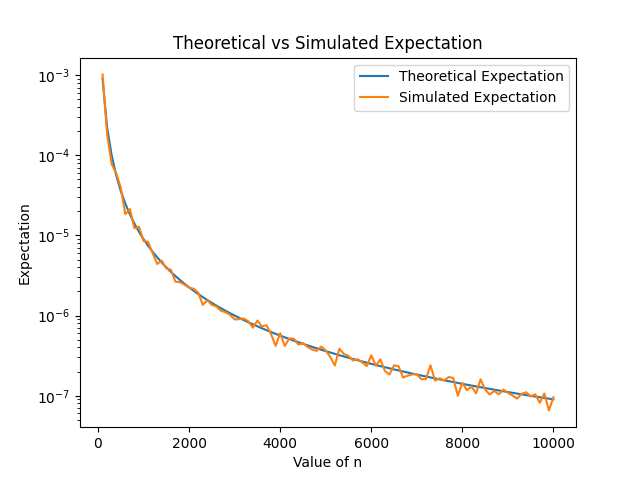
\includegraphics[width=\columnwidth]{figures/expectation.png}
    \caption{Expectation vs n}
    \label{fig:st_2023_32_figure}
\end{figure}
In both cases, we can observe the limit tends towards zero.
\end{enumerate}
\end{document}  
\end{enumerate}
